
\cleardoublepage
\chapter*{Introduction}
\markboth{that separateon}{Introduction}
\addcontentsline{toc}{chapter}{Introduction}

While the sun is essential to the income of energy on earth, the solar flares would tear off its atmosphere if there was not the protecting magnetosphere to act as planetary shield. Nevertheless geomagnetic storm or substorm are disturbances that can make its tail change, and that generate due to a reconnection process in the magnetic field lines, and can be shown as beautiful auroras. The matter in solar flares, and in fact in all the universe is manly in a plasma state, meaning that it is ionized and follows the magnetic field, which is why the magnetosphere acts nicely as a shield !

On Earth, a good understanding of the magnetic topology is essential to achieve a controlled fusion process in a reactor device. The electromagnetic fields determine to a great extent the evolution of the plasma, making it well or poorly confined. Although fusion can also be achieved by inertial confinement, which is currently the subject of research, it is not quite as mature as the concept of magnetically confined plasma for fusion. Several different geometric designs have been explored, and the attempt to confine the plasma in a toroidal shape has proved most promising. A stability condition for good confinement is that the field must twist, causing the particles to move between low and high radii, effectively rotating around the axis of the torus. 

This twisting is at the root of a schism in the design of toroidal magnetic fusion devices, leading to the two well known : Stellarator and Tokamak concepts. Both concepts involve a magnetic field that is simultaneously toroidal and poloidal, rotating around the torus and around a particular field line called the magnetic axis. The toroidal component of the magnetic field is generated by the use of coils. They differ in the way the poloidal field is produced: Tokamaks induce a current in the plasma, which then generates the poloidal component according to Ampere's law. Stellarators have coils formed directly into modular shapes, eliminating the need for a net current, but are much more difficult to engineer and construct.


In stellarators design, the magnetic topology has more freedom than for tokamaks. In fact, there are an infinite number of possible configurations. A type of divertor then exploits a resonance due to the winding of the field line to create magnetic islands at specific locations in the edge region, which channels the heat flux to specific locations in the plasma-facing components. \cite{feng_review_2022} reviews the divertor-relevant geometric parameters of the magnetic island divertor in the W7X stellarator. A transport model is presented that can be employed to design a divertor in a W7-X with tungsten instead of graphite. 

Another type of divertor is the non-resonant divertor (NRD). An NRD would be placed in trough regions : configuration-specific `toroidal ridges' where the field lines primarily escape \cite{bader_hsx_2017}.\cite{garcia_exploration_2023} study the edge structure in the Compact Toroidal Hybrid device by looking at the connection length, the travelled distance before hitting a PFC. They describe the striking patterns on a hypothetical divertor for different currents and at different divertor positions, using the EMC3-EIRENE 3D code, and link it to chaos. They calculate the heat flux and Mach number and draw a parallel with the chaotic structure present in another type of divertor, the ergodic divertor. An NRD, unlike a resonant divertor, would not be subject to the position of a particular low order island, which can be affected by the generated field/currents of the plasma motion itself. A NRD can therefore be a more robust design.

The stochasticity present in magnetically confined devices, described in great detail by \cite{abdullaev_magnetic_2014}, leads to a third type of divertor concept, the ergodic divertor. Originally used to correct inaccuracies in toroidal coils that cause a non-axisymmetric field in tokamaks, resonant magnetic perturbation coils can also introduce mixing in the field line at the edge, which has been found to be beneficial for mitigating ELMs, a type of instability inherent to the high confinement regime in which, for example, the future DEMO reactor is designed to operate. The RMP coils are discussed as a means of creating an ergodic region in the edge, controlling the heat and particle fluxes, and directing the particles towards the divertor plates. The ergodic divertors have been used and studied in the WEST (formerly Tore Supra) and TEXTOR tokamaks.

The study of the edge plasma region is then essential for the design of a reliable divertors. As \cite{imbert-gerard_introduction_2020} nicely points out, the complexity of describing the processes in a plasma can be tackled by considering different models depending on the length and time scale. Without taking into account the gyroscopic motion of the charged particles around the magnetic field and neglecting the interaction between the particles and the fields still provide a way to distinguish between different regions of the plasma in the stellarator. Following the movement of a point in the direction of $\textbf{B}$ (forward) or $-\textbf{B}$ (backward) gives a field line and is called field line tracing (FLT). It is usually used to draw the intersections or to view the connection length plot and provides significant amount of information about a configuration.

In the more general case of a 3 dimensional vector field, \cite{wei_invariant_2023} describes the FLT in cylindrical coordinates as a map that shows the evolution of the crossing of a field line with a constant toroidal angle semi-plane. The resulting map, which I will call the field line or Poincaré map,  is shown to have a determinant related to the divergence of the vector field. If the configuration is chaotic, then the trajectories depend strongly on the initial conditions, and two almost indistinguishably close initial conditions will eventually evolve into noticeably different regions of phase space. H. Poincaré was a precursor in this regard, looking at chaos in the case of celestial mechanics for the three-body problem. He associated chaotic behaviour with the appearance of an infinitely refined lattice structure, which he called a trellis in analogy with the construction of the interconnected garden fence \cite[Ch.33]{poincare_methodes_1892}. The trellis structure arises when looking at some specific points in periodic orbits and is formed by the interconnection of two curves, the unstable and the stable manifold of one or more hyperbolic fixed point. Nowadays it is also called a tangle.

As \cite{wei_invariant_2023} put it : "With the aid of modern dynamical system theory, the structure of a 3D vector field can be comprehended and analyzed in terms of invariant manifolds". In their paper they then show a hypothetical tangle in the case of an EAST shot when an RMP induced field would be added. In the case of field line tracing, we can analyse the 3-dimensional manifolds and tangle structure in a cross section with the field line map.

The field line map is continuous, but is a non-trivial problem: there is no general analytical formula, it can be lengthy to perform FLT, and the integration is prone to error. These difficulties make the study of the field line map not the best playground for understanding chaos.  Simpler analytical maps are then a nice way to still study chaos, and in particular the symmetric and asymmetric Tokamaps have been introduce to describe FLT in Tokamaks \cite{abdullaev_mappings_2006}. There are based on a continous Hamiltonian system which consists in an integrable part specified by the winding profile, more precisely the safety factor $q$ profile, and a non-integrable perturbation. \figref{fig:tokamap} shows the orbits of the symmetric tokamap for a monotonic $q$ profile and perturbed. We can clearly see the difference between the region where the field lines form closed surfaces, the magnetic islands, and the regions where the points get mixed up, the chaotic zone. In fact, there may still remain some invariant tori in the chaotic sea. They are called cantori and there existence is proven by the KAM theorem.

\begin{figure}[h!]
    \centering
    \begin{subfigure}[t]{0.43\textwidth}
        \centering
        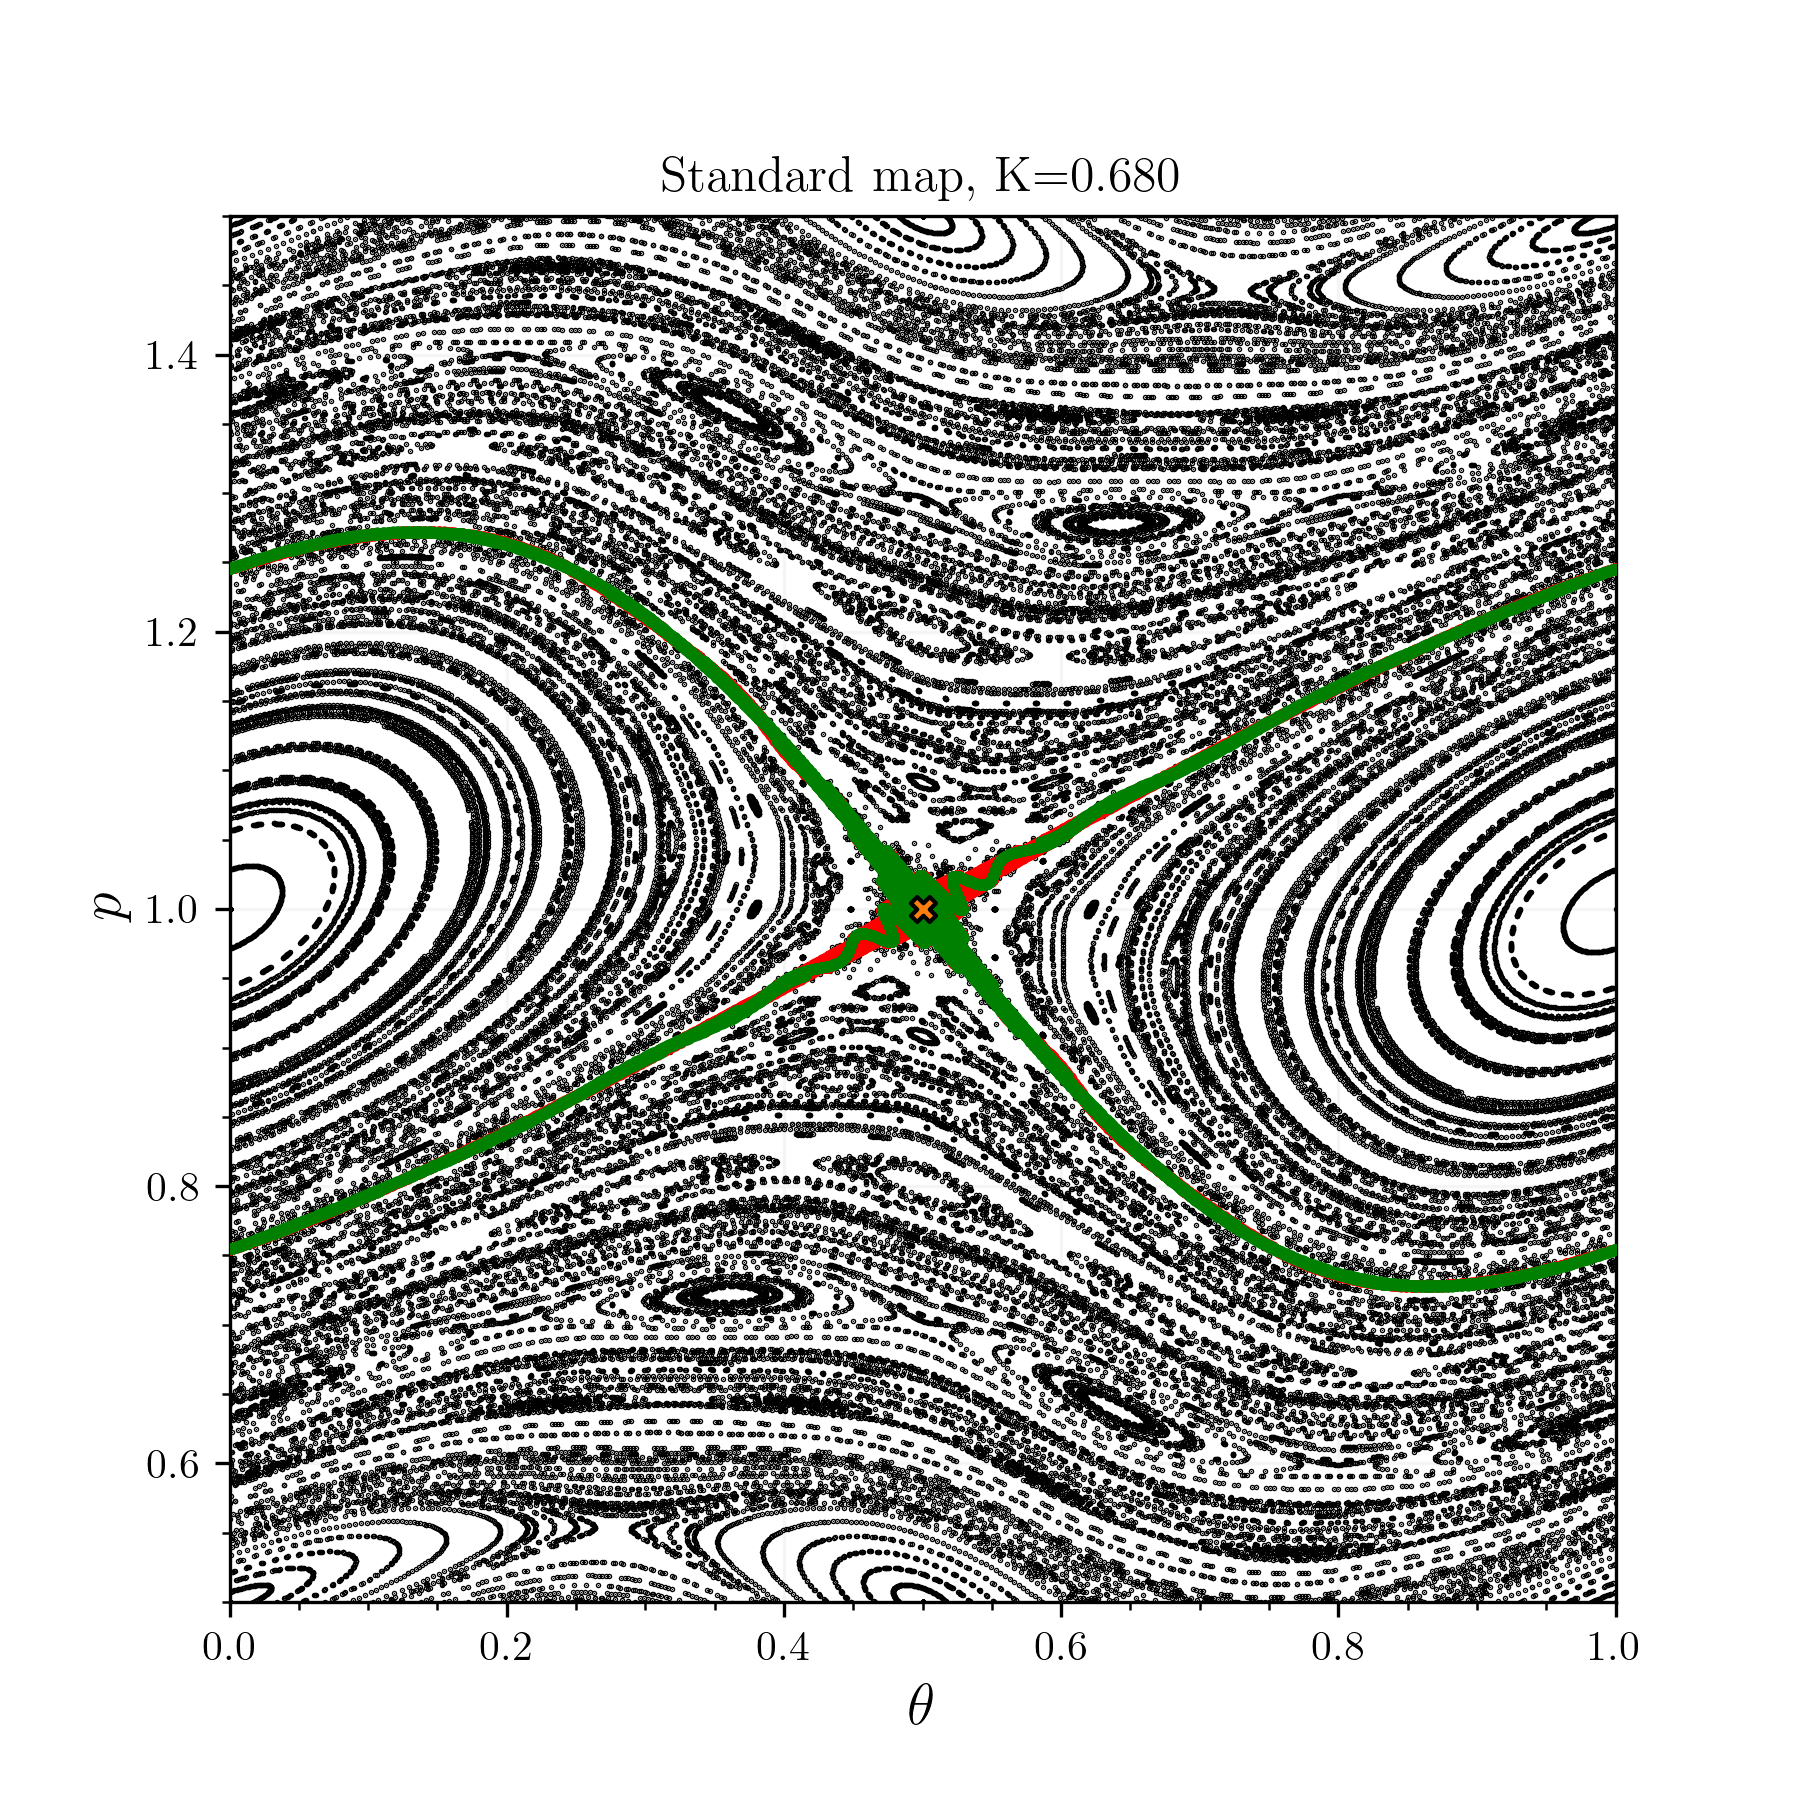
\includegraphics[width=\textwidth]{images/intro/manifold_0.680_28.png}
        \caption{}
        \label{fig:standard-map}
    \end{subfigure}
    \hfill
    \begin{subfigure}[t]{0.56\textwidth}
        \centering
        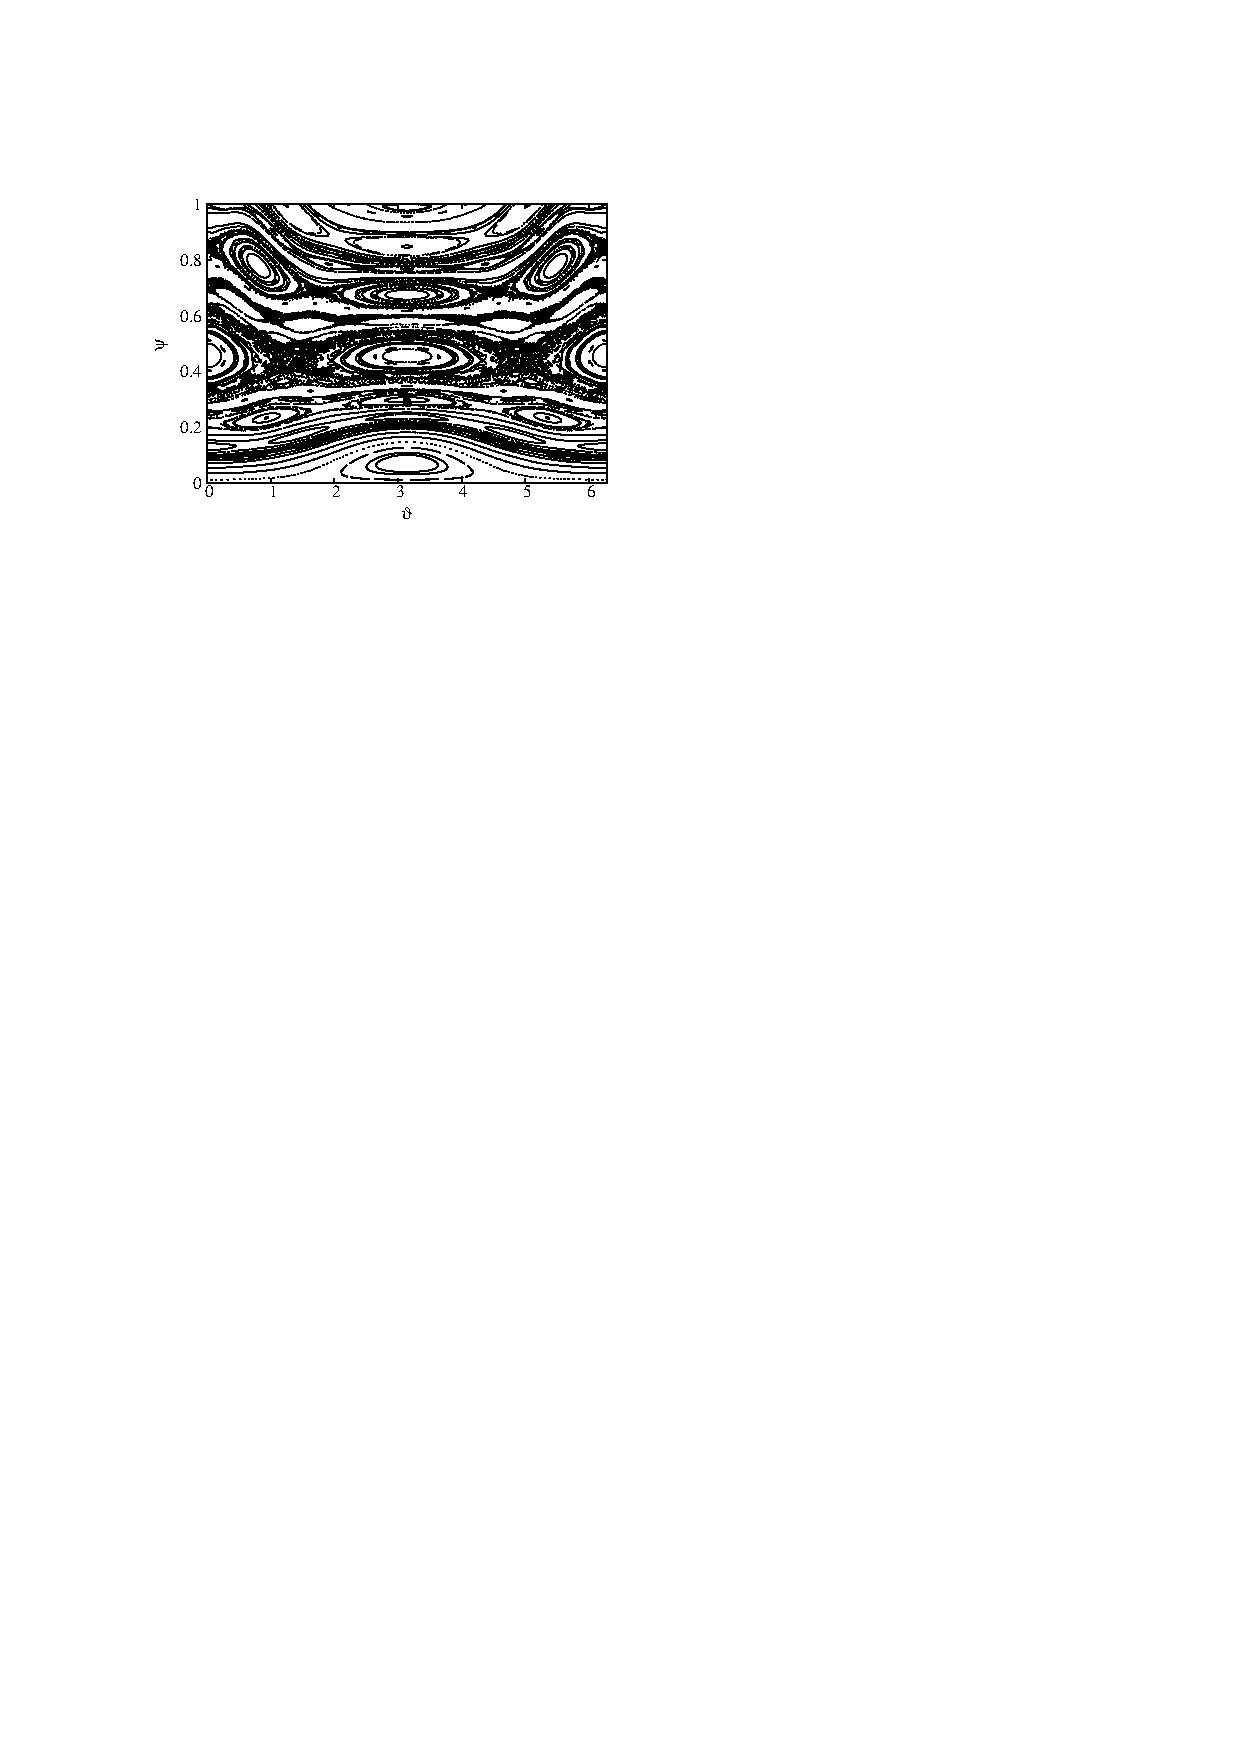
\includegraphics[width=\textwidth]{images/intro/tokamap.pdf}
        \caption{}
        \label{fig:tokamap}
    \end{subfigure}
    \caption{Map for which the chaos is more easily studied and with similar behaviour as field line tracing~: (a) standard map on the cylinder for the parameter $K=0.68$. (b) symmetric tokamap taken from \cite{wingen_stochastic_2005}.}
    \label{fig:mapping-the-chaos}
\end{figure}

For more 
\cite{meiss_thirty_2015} enlightens the progress that has been made in the characterization of transport for a deterministic dynamical system. Theoretical foundations in the context of volume-preserving maps (and therefore sympletic maps) are laid out ; the stable and unstable manifold of hyperbolic points bound resonance regions and their primary intersections, hetero/homo-clinic points, play an important role in determining the exiting/incoming fluxes. Inside chaotic layers, cantori are partial barriers separating orbits of the chaotic sea. Transition times are discussed and the fat fractal mixing of the islands for the Henon map is tackled down by considering a Markov chain decomposition.

"It is important to note that one of the fundamental measures of chaos, the Lyapunov exponent is not usually a good measure for transport. In Ref. 86, we said: The Lyapunov exponents give the rate at which a nice cat in a region of phase space turns into a mixed-up cat. The turnstile rate constants give the mean rate at which bits of the cat are transported to regions of the phase space"


--------
\\[10pt]
transoprt through chaos \cite{easton_transport_1991}
\\[10pt]

Those have been experimentaly observed in

\\[10pt]
Magnetic turnstiles in nonresonant stellarator divertor
\\[10pt]

\\[10pt]
experimental signatures of homoclinic tangles \cite{evans_experimental_2005}
\\[10pt]